\chapter{مزایا و کاربردهای \lr{IMS}}
 \setlatintextfont{Times New Roman}
 \label{benefitsPart}
\section{کاهش هزینه\nf ها، افزایش درآمد و رفع وابستگی}

ارائه\nf ی سروریس\nf های جدید، سودآورترین عامل در استفاده از \lr{IMS} است. پیاده\nf سازی \lr{IMS}، باعث کاهش هزینه\nf های عملیّاتی و هزینه\nf های مربوط به شبکه می\nf شود و برای اپراتورها، سودآور است\RTLfootnote{پروژه\nf ی \lr{clearwater} ادّعا می\nf کند که در صورت استفاده از ابر آمازون به\nf عنوان بستر پیاده\nf سازی \lr{IMS} توسّط این پروژه، این هزینه به\nf ازای هر کاربر در طول یک سال، برابر دو سنت(دو صدم دلار) است.}. همچنین، کاهش زمانِ بین طرّاحی اپلیکشین\nf های جدید و ارائه آن\nf ها به مشترکین، از دیگر عوامل سودآوری است. شکل \ref{cost}، سهم هر یک از عوامل فوق را در سودآوری برای اپراتورهای تلفن همراه نشان می\nf دهد\cite{blended}.

\begin{figure}[h]
\centering
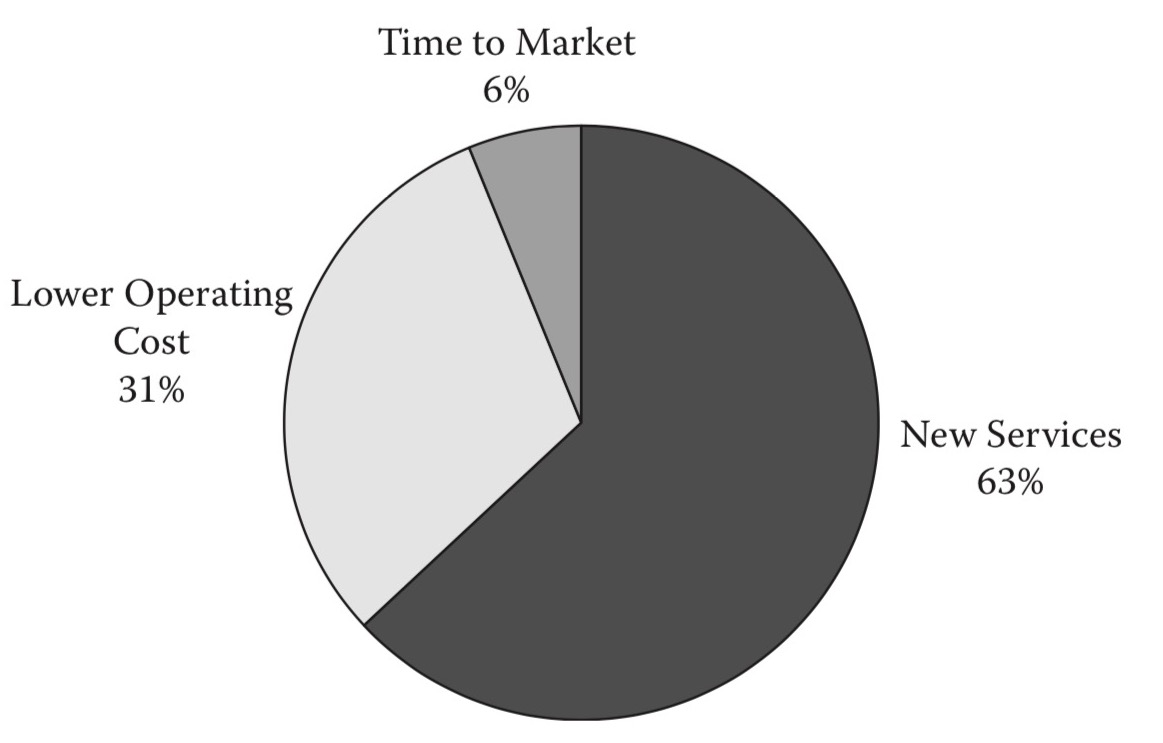
\includegraphics[width=0.68\textwidth]{cost}
\caption{مقایسه\nf ی میزان سودآوری عوامل مختلف پس از پیاده\nf سازی \lr{IMS}}
\label{cost}
\end{figure}

\subsection{جایگزین سوئیچ\nf های مداری}
\begin{figure}[h]
\centering
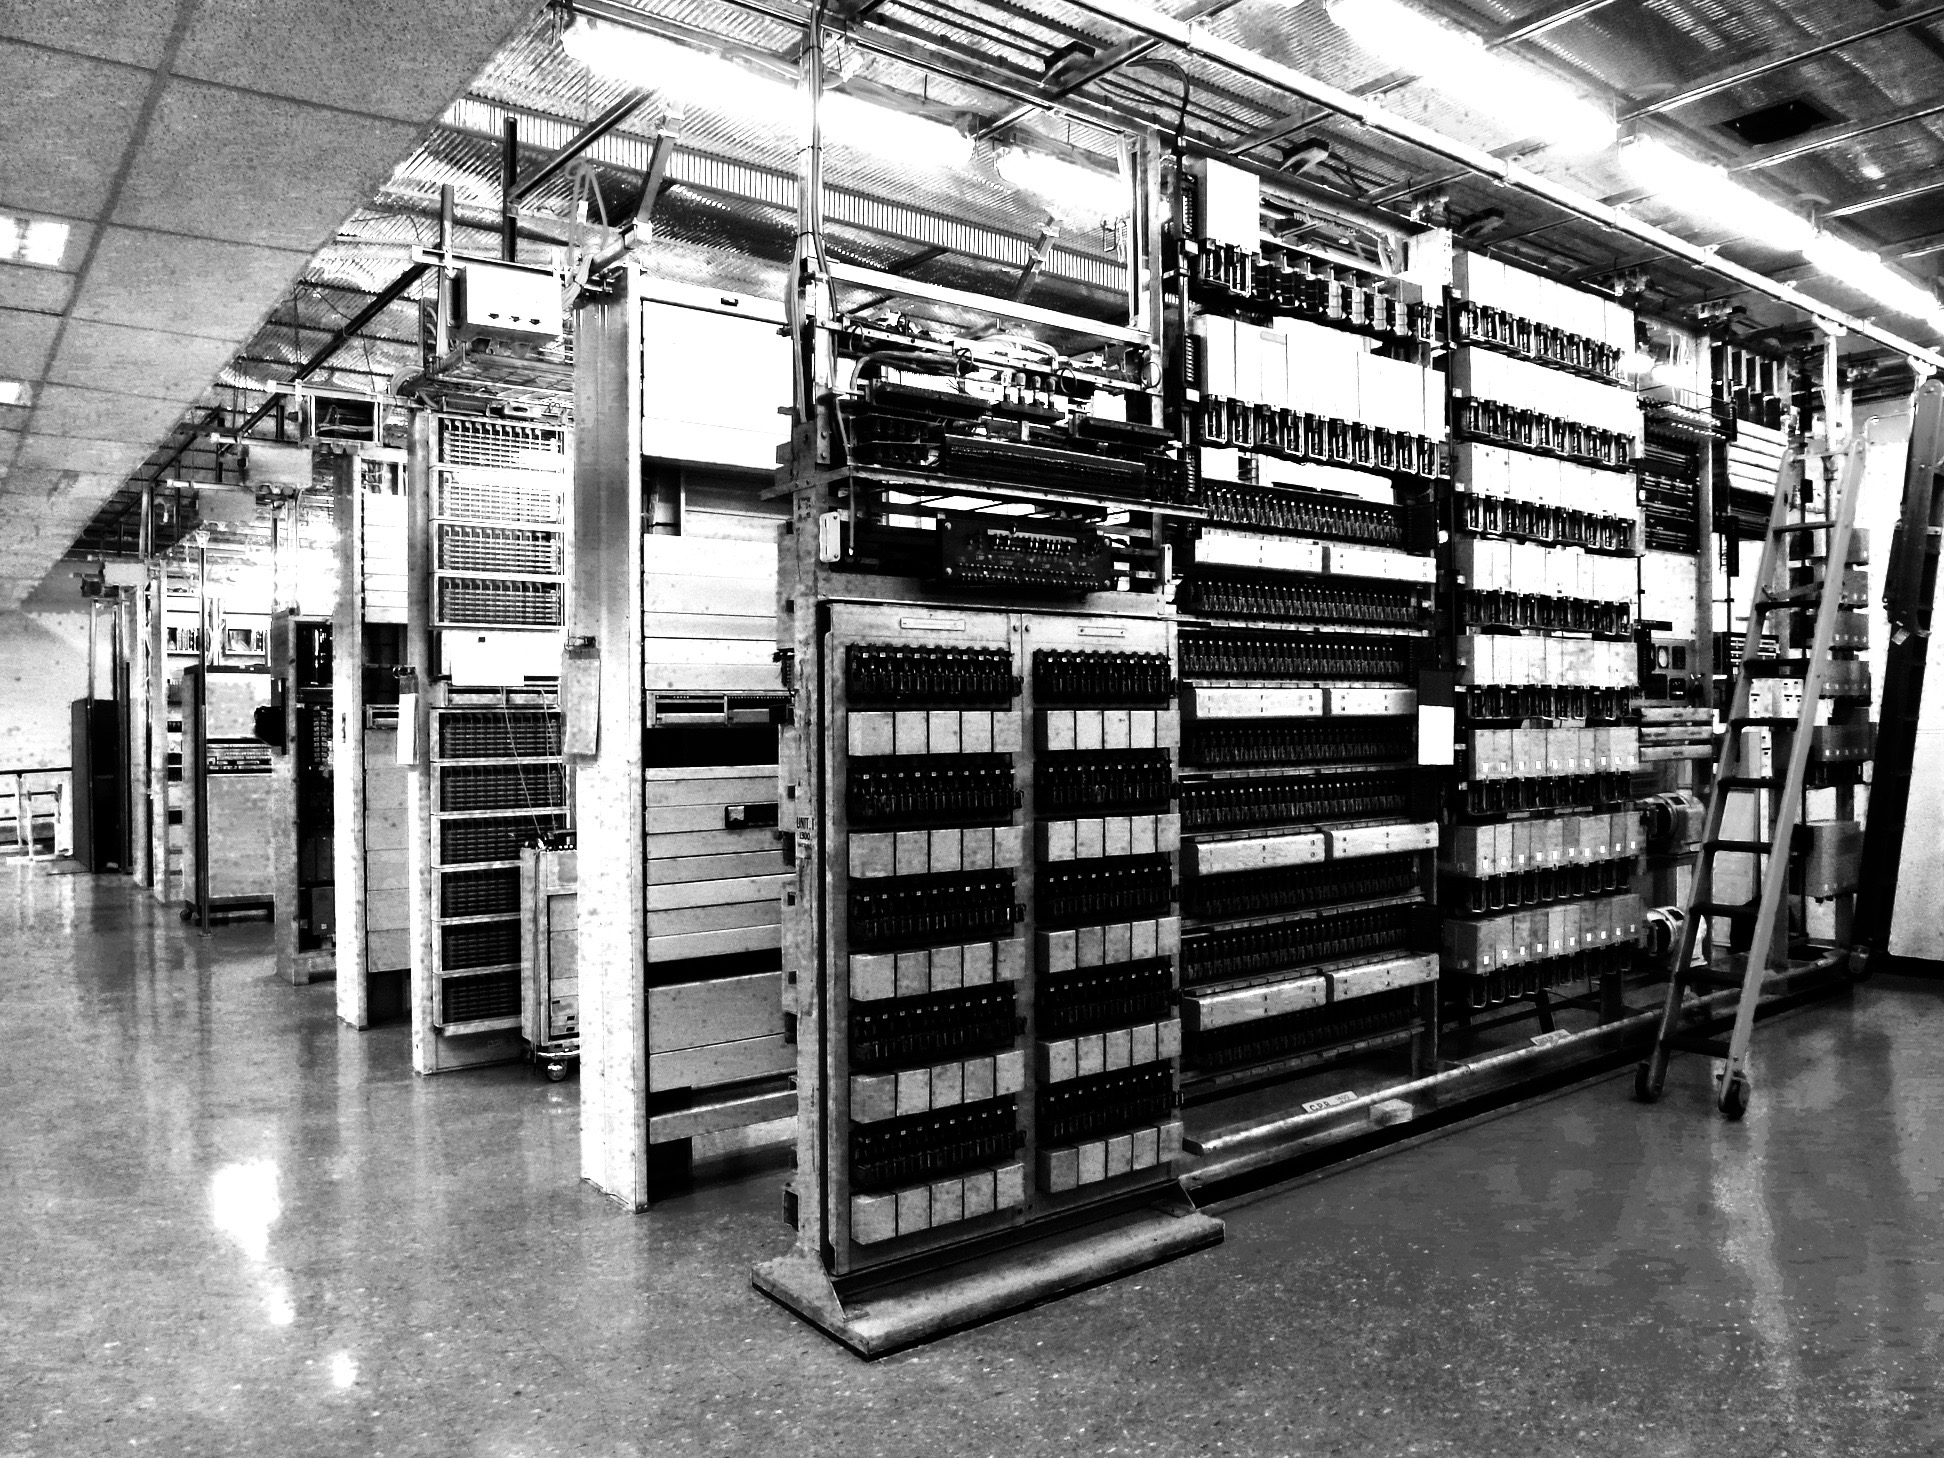
\includegraphics[width=0.7\textwidth]{cs}
\caption{نمایی از سوئیچ\nf های مداری که در مراکز تلفن و مراکز سوئیچینگ تلفن همراه به\nf کار می\nf رود}
\label{cs}
\end{figure}

از آنجایی\nf که سوئیچ\nf های مداری به\nf صورت سخت\nf افزاری پیاده\nf سازی شده\nf اند، هزینه\nf ی بالایی دارند. همچنین، با زیاد شدن تعداد مشترکین، لازم است که تعداد سوئیچ\nf های مداری افزایش یابد. از این رو جایگزین کردن این سوئیچ\nf ها با سوئیچ\nf های بسته\nf ای بسیار مقرون به صرفه است؛ زیرا  سوئیچ\nf های بسته\nf ای می\nf توانند با هزینه\nf ی کمتری نسبت به سوئیچ\nf های مداری، به کاربران بیشتری سرویس ارائه کنند.

 به دلیل تولید سوئیچ\nf های مداری توسّط شرکت\nf های خارجی نظیر شرکت اریکسون و مشکلاتی نظیر تحریم\nf ها، حذف این سوئیچ\nf ها قدمی بزرگ به سمت خودکفایی صنعت مخابرات به\nf شمار می\nf رود. از آنجایی\nf که سوئیچ\nf های مداری، به\nf صورت تجاری عرضه می\nf شوند و برخی شرکت \nf های داخلی نیز قادر به تولید آن\nf ها می\nf باشند، وجود تحریم\nf ها مانعی برای استفاده از آن\nf ها به شمار نمی\nf رود.
 

\subsection{آسان کردن ارائه\nf ی سرویس\nf های نوظهور}
\label{benefits1}

در نسل دوّم ارتباطات، ایجاد یک سرویس جدید مانند سرویس پیامک، دو تا سه سال زمان می\nf بُرد. با ظهور نسل سوّم ارتباطات و بهبود زیرساخت\nf ها، این زمان به حدود ۶ ماه کاهش یافت. با ظهور \lr{IMS}، می\nf توان در مدّت چند روز تا حداکثر چند هفته، اپلیکیشن طرّاحی\nf شده را به شبکه اضافه کرد و سرویس موردنظر را در اختیار کاربران قرار داد.

دلیل اوّلِ این موضوع، وجود رابط\nf های برنامه\nf نویسی اپلیکشن\RTLfootnote{\lr{Application Programming Interface(API)}} در تمام نقاط معماری \lr{IMS} است. لذا، نیاز نیست که برای هر اپلیکیشن جدیدی که قرار است به\nf کار برده شود، روش\nf های مستقرسازی\RTLfootnote{\lr{deployment}} خاص مورد استفاده قرار گیرد. مثلاً اپلیکیشن جدید می\nf تواند به\nf راحتی و با استفاده از ابط\nf های برنامه\nf نویسی اپلیکشن، با المان \lr{CDF}\RTLfootnote{سرواژه\nf ی عبارت \lr{Charging Date Function}. این المان، برای ارائه\nf ی خدمات شارژ و کنترل مالی حساب مشترکین به\nf کار می\nf رود.} ارتباط برقرار کند و هزینه\nf ی سرویسی را که به مشترک ارائه می\nf کند، از حساب او کم کند\cite{blended}.

دلیل دوّم، لایه\nf ی \lr{enabler} می\nf باشد که به\nf عنوان بخشی از لایه\nf ی اپلیکیشن تعریف شده است و اطّلاعت خاص شبکه را برای اپلیکیشن\nf ها فراهم می\nf کند. \lr{enabler}، یک تابع خاص است که یک بار در شبکه اجرا می\nf شود و اطّلاعاتش بین چندین اپلیکیشن به اشتراک گذاشته می\nf شود. این اشتراک\nf گذاری، به دلیل افزایش کارایی، کاهش هزینه\nf ها و همچنین ایجاد امکان به اشتراک گذاشتن اطّلاعات اشتراکی بین اپلیکیشن\nf های مختلف مورد استفاده قرار می\nf گیرد. در شرایطی که سیستم\nf های کنونی، از روش ستونی\RTLfootnote{به دلیل شباهت شکل ستون به سیلوی غلّات، به روش ستونی، روش سیلو نیز می\nf گویند. } برای در اختیار قرار دادن اطّلاعات شبکه به اپلیکیشن\nf ها استفاده می\nf کنند، \lr{IMS} با استفاده از  \lr{enabler} های اشتراکی، نیاز به استفاده از سرورهای مجزّا برای این کار را رفع می\nf کند\cite{blended}.

\begin{figure}[h]
\centering
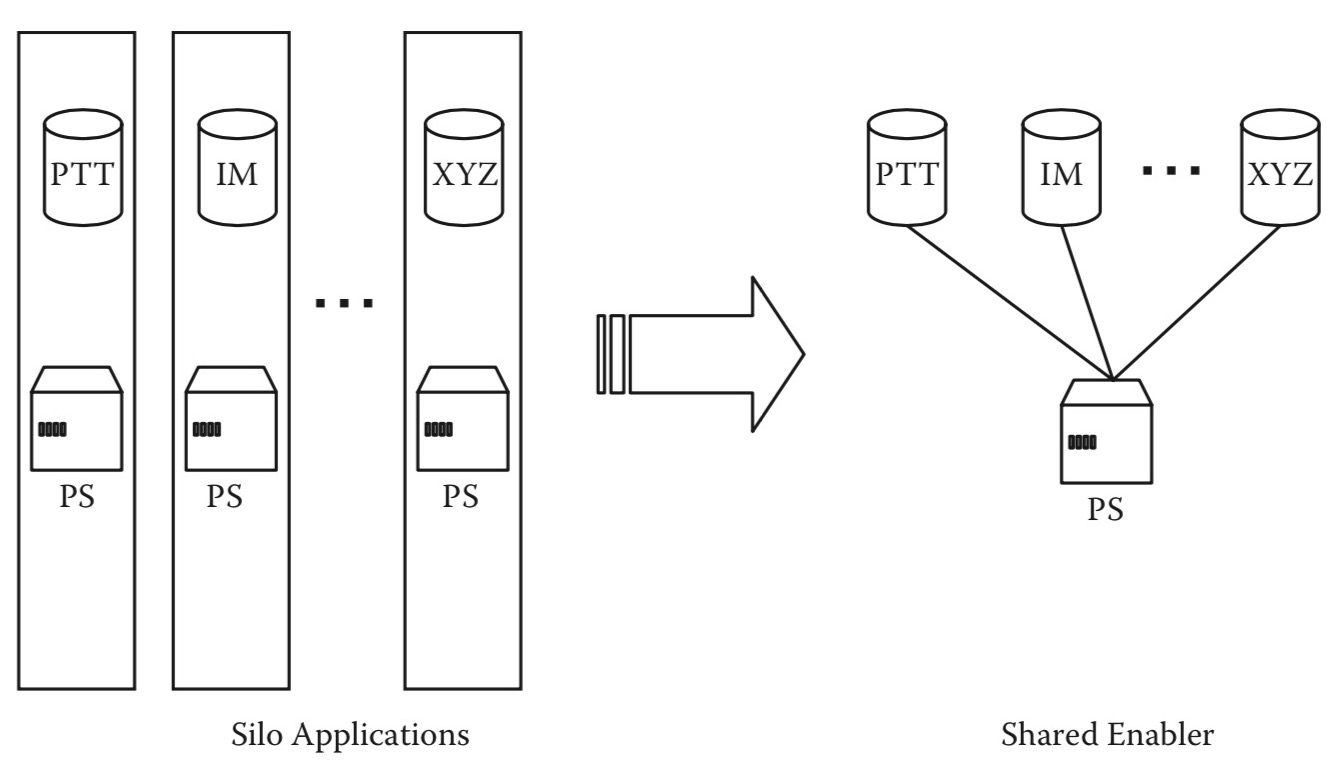
\includegraphics[width=0.7\textwidth]{enabler}
\caption{استفاده از روش ستونی و روش \lr{enabler} مشترک}
\label{enabler}
\end{figure}

به\nf عنوان مثال، سرویس\nf های \lr{PTT}\RTLfootnote{\lr{Push To Talk}: سرویسی است که امکان استفاده از تلفن همراه به عنوان بیسیم\nf های مخابراتی را فراهم می\nf کند. در واقع، ارتباط مشترکین این سرویس در هنگام تماس، به\nf گونه\nf ای است که در هر لحظه، فقط یک نفر می\nf تواند صحبت کند.} و پیامک\RTLfootnote{\lr{Instant Messaging}}، هر دو نیاز دارند که از وضعیت حضور مشترکین در شبکه آگاه باشند. در سیستم\nf های متداول امروزی، هر کدام از این اپلیکیشن سرورها، از سرور وضعیت\RTLfootnote{\lr{Presence Server}} مخصوص به خود استفاده می\nf کنند و امکان به اشتراک گذاشتن وضعیت حضور مشترکین سرویس \lr{PTT} با اپلیکیشن سرور پیامک وجود ندارد. امّا هنگامی که از یک \lr{enabler} مشترک استفاده شود، تنها با استفاده از یک سرور وضعیت می\nf توان اطّلاعات مربوط به وضعیت حضور مشترکین را هم\nf زمان در اختیار اپلیکیشن سرور پیامک و اپلیکیشن سرور \lr{PTT} و سایر اپلیکیشن سرورها قرار دارد(شکل \ref{enabler}). در صورتی که لازم باشد یک اپلیکیشن سرور جدید برای کاربردی نوظهور به شبکه اضافه شود و این اپلیکیشن سرور، نیاز به دانستن وضعیت حضور مشترکین داشته باشد، بدون نیاز به ساخت و راه\nf اندازی یک سرور وضعیت جدید می\nf توان از سرور وضعیت موجود در شبکه استفاده کرد. به این ترتیب، زمان و هزینه\nf ی پیاده\nf سازی اپلیکیشن سرورهای جدید و ارائه\nf ی کاربردهای نوظهور، کاهش میابد\cite{blended}.

\section{ورود شرکت\nf های شخص ثالث به بازار مخابرات}
با توجّه به مطالب بیان\nf شده در بخش \ref{benefits1}، استفاده از \lr{IMS} باعث کاهش زمان، پیچیدگی پیاده\nf  سازی و هزینه\nf ی ایجاد اپلیکیشن سرور و ارائه\nf ی سرویس\nf های نوظهور می\nf شود. این موضوع باعث هموار شدن راه سایر شرکت\nf ها برای ورود به بازار مخابراب به\nf عنوان شرکت\nf های شخص ثالث می\nf شود.

\subsubsection{طرّاحی و فروش اپلیکیشن سرور}

شرکت\nf های شخص ثالث می\nf توانند اپلیکیشن سرورهای جدید برای ارائه\nf ی کاربردهای نوظهور طرّاحی کنند و  این اپلیکیشن سرورها را به اپراتورهای تلفن همراه بفروشند. به دلیل آسان\nf تر شدن پیاده\nf سازی و راه\nf اندازی اپلیکیشن سرورها در صورت استفاده از \lr{IMS}، اپراتورهای تلفن همراه استقبال بیشتری از این موضوع خواهند کرد. همچنین، کاهش زمانِ بین طرّاحی اپلیکیشن سرور و ارائه\nf ی سرویس جدید به کاربران، باعث می\nf شود که طرح\nf های جدید، زودتر به سودآوری برسند. این موضوع، هم برای شرکت\nf های شخص ثالث و هم برای اپراتورهای تلفن همراه حائز اهمیّت است. 

\subsubsection{استفاده از زیرساخت اپراتورهای تلفن همراه}

زیرساختی که اپراتورهای تلفن همراه برای ارائه\nf ی سرویس خود ایجاد کرده\nf اند، به\nf طور کامل مورد استفاده قرار نمی\nf گیرد و این قابلیت را دارد که سرویس\nf های بیشتری را به کاربران بیشتری ارائه دهد. وجود درگاه \lr{OSA}(بخش \ref{osapart})، این امکان را فراهم می\nf کند که شرکت\nf های نوظهور بتوانند سرویس\nf های خود را با استفاده از زیرساخت اپراتورها ارائه کنند.

\nf 
\section{ عدم وابستگی به شبکه\nf ی دسترسی }

\subsubsection{استفاده از شبکه\nf های محلّی و اینترنت}

از ویژگی\nf های اصلی \lr{IMS}، عدم وابستگی به شبکه\nf ی دسترسی\RTLfootnote{\lr{Access Network Independent}} می\nf باشد. این ویژگی باعث می\nf شود که کاربر بتواند از طریق اتّصال به سایر شبکه\nf ها، از سرویس \lr{IMS} بهره\nf مند شود. مشترکین اپراتور، می\nf توانند با اتّصال تلفن همراه خود به شبکه\nf ی اینترنت(از طریق وای\nf فای)، از خدمات اپراتور خود و \lr{IMS} بهره\nf مند شوند. استفاده از وای\nf فای به\nf جای ارتباط با ایستگاه مخابراتی، مزایای زیادی دارد. این کار باعث کاهش مصرف باتری تلفن همراه و صرفه\nf جویی در مصرف برق می\nf شود\RTLfootnote{ارتباط وای\nf فای، توان کمتری نسبت به ارتباطات مخابرات سلولی مصرف می\nf کند.}. همچنین به دلیل کاهش سیگنال\nf های مخابراتی که کاربر به ایستگاه\nf های مخابراتی می\nf فرستد، ضررهای ناشی از این سیگنال\nf ها کاهش خواهد یافت\RTLfootnote{به دلیل پایین\nf تر بودن دامنه\nf ی فرکانسی وای\nf فای نسبت به امواج مورد استفاده در ارتباط با ایستگاه مخابراتی، ضررهای جسمانی کم\nf تری به بدن انسان می\nf رسد.}.

به دلیل عدم وابستگی \lr{IMS} به شبکه\nf ی دسترسی، دیگر الزامی نیست که مشترکین تلفن همراه برای برقراری تماس تلفنی، به ایستگاه\nf های مخابراتی متّصل شود. لذا در نقاطی که پوشش آنتن\nf دهی مناسبی وجود ندارد، مشترکین می\nf توانند با استفاده از شبکه\nf ی اینترنت\RTLfootnote{اینترنتی که توسّط فیبر نوری و یا کابل تلفن ثابت در اختیار آن\nf ها قرار می\nf گیرد و عموماً به\nf صورت سرویس \lr{ADSL} است.} خود از خدمات اپراتور تلفن همراه خود بهره\nf مند شوند. همچنین، این امکان وجود دارد که اپراتورهای تلفن همراه به\nf جای ساخت ایستگاه مخابراتی در نقاط دور دست(که بسیار هزینه\nf بر است)، یک شبکه\nf ی محلّی مبتنی بر پروتکل اینترنت در آن مناطق ایجاد کنند. با اتّصال این شبکه\nf ی محلّی به شبکه\nf ی داخلی اپراتور،کاربران قادر به استفاده از خدمات \lr{IMS} و اپراتور موردنظر می\nf شوند.

\begin{figure}[h]
\centering
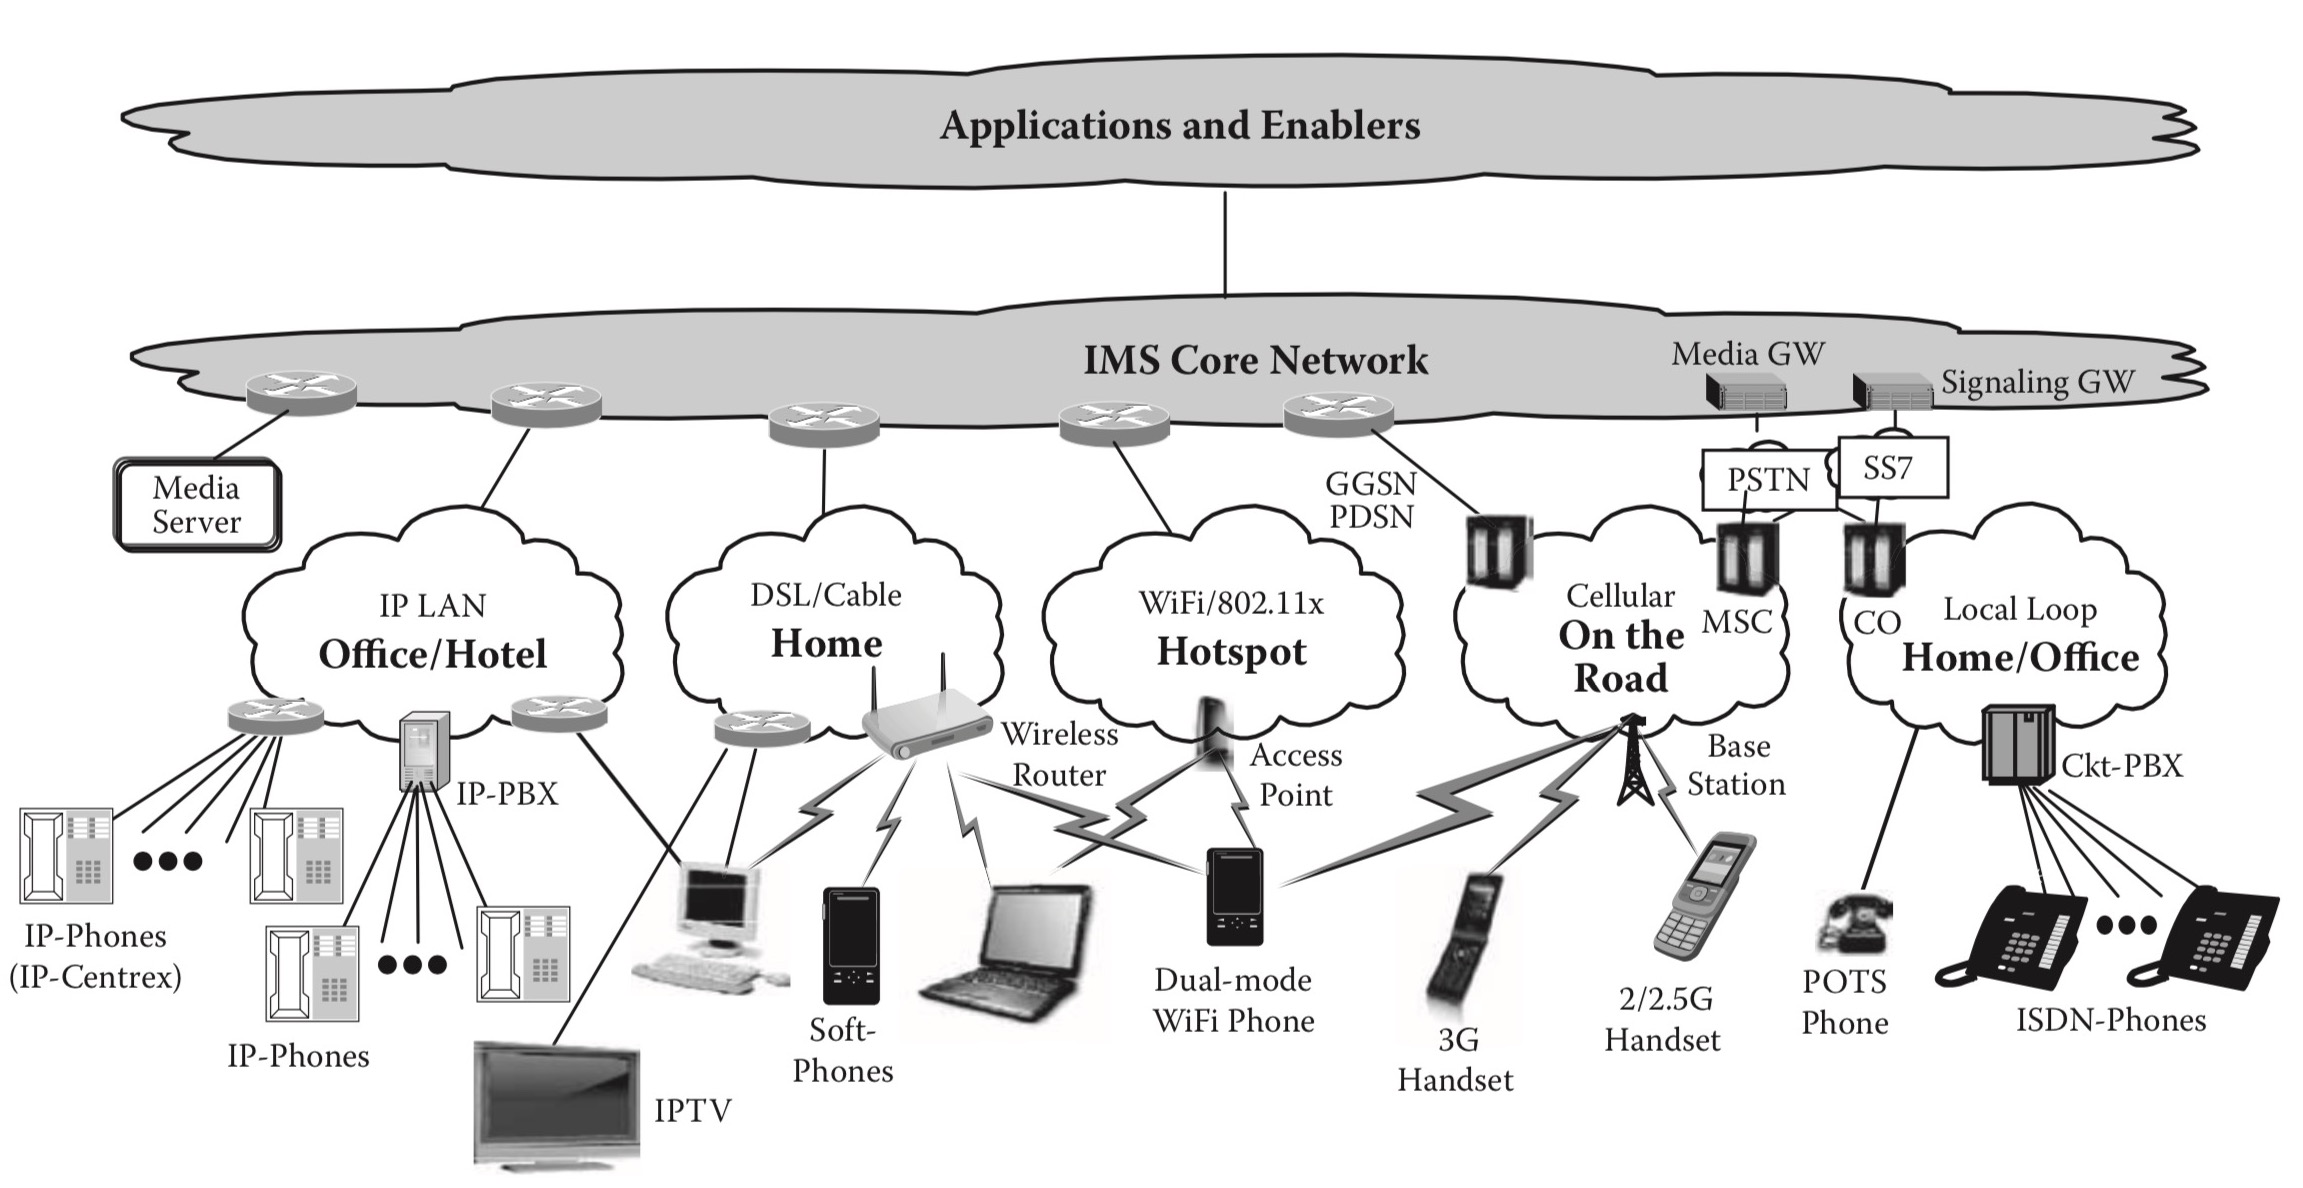
\includegraphics[width=\textwidth]{accessin}
\caption{پشتیبانی از شبکه\nf های دسترسی مختلف توسّط \lr{IMS}}
\label{accessin}
\end{figure}

\subsubsection{اتّصال با دستگاه\nf های مختلف}

در \lr{IMS}، این امکان وجود دارد که با دستگاه\nf های مختلف به شبکه\nf ی اینترنت متّصل شد و سپس از خدمات اپراتور مربوطه و \lr{IMS} مانند تماس صوتی، بهره\nf مند شد. از آنجایی\nf که \lr{IMS} به شبکه\nf ی دسترسی وابستگی ندارد، کاربر می\nf تواند با دستگاه\nf هایی نظیر کامپیوتر شخصی خود به اینترنت متّصل شده و از طریق آن، تماس صوتی برقرار نماید. البتّه لازم است که تدابیری برای ایجاد این قابلیت اندیشیده شود. استفاده از یک رمزعبور اختصاصی برای هر کاربر، لازمه\nf ی این کار است. همچنین، این امکان وجود دارد که کاربر با یک شماره تلفن، هم\nf زمان از طریق چند دستگاه به شبکه\nf ی اپراتور موردنظر خود متّصل شود\cite{3gims}.

\subsubsection{جابه\nf جایی}
سیستم \lr{IMS}، این قابلیت را دارد که سطح بالاتری از جابه\nf جایی\RTLfootnote{Mobility} را به کاربران خود ارائه دهد. در سیستم\nf های گذشته، کاربران می\nf توانستند به مکان\nf های جغرافیایی مختلف بروند و به ایستگاه\nf های مخابراتی مختلف اپراتور خود متّصل شوند، بدون این که ارتباط آن\nf ها قطع شود. سطح بالاتر جابه\nf جایی که رومینگ\RTLfootnote{\lr{Roaming}} نام دارد، اتّصال دستگاه کاربر به ایستگاه\nf های مخابراتیِ سایر اپراتورها و دریافت سرویس اپراتور خود، از طریق این ایستگاه\nf ها می\nf باشد. سطح بالاتری از جابه\nf جایی که توسّط \lr{IMS} ارائه می\nf شود، اتّصال کاربر به شبکه\nf های دسترسی متفاوت و دریافت سرویس از اپراتور خود است. با وجود تغییر شبکه\nf ی دسترسی کاربر، ارتباط کاربر قطع نخواهدشد و کاربر قادر است به\nf راحتی و بدون قطع ارتباط، بین شبکه\nf های دسترسی مختلف جابه\nf جا شود\cite{blended}.



\section{کاربردهای نوظهور}
کاربردهای نوظهور بسیاری توسّط سیستم \lr{IMS} فراهم می\nf شوند که در اینجا، چند مورد از مهم\nf ترینِ آن\nf ها ذکر شده\nf اند. برای مطالعه\nf ی بیشتر، به \cite{blended} و \cite{3gims} مراجعه شود.

\subsubsection{تماس ویدیوئی و کنفرانس صوتی و ویدوئی}

از آنجایی\nf که \lr{IMS}  مبتنی بر پروتکل \lr{SIP} است، می\nf توان به\nf وسیله\nf ی آن تماس ویدیوئی برقرار کرد. همچنین، امکان ایجاد یک جلسه بین چند کاربر و برقراری کنفرانس صوتی و ویدوئی نیز وجود دارد. از آنجایی\nf که در بسیاری از مواقع، کاربران \lr{IMS} به شبکه\nf ی داخلی اپراتور تلفن همراه خود متّصل هستند، هزینه\nf ی تماس ویدیوئی و یا برقراری کنفرانس(صوتی یا ویدیوئی) نسبت به سیستم\nf های کنونی ارزان\nf تر خواهد بود\cite{blended}. 


\subsubsection{\lr{IP messaging}}

از دیگر قابلیت\nf های \lr{IMS}، فراهم کردن سرویس غنی ارتبطات است\RTLfootnote{\lr{Rich Communication Service(RCS)}}. سیستم \lr{IMS} این قابلیت را دارد که سرویسی مشابه اپلیکیشن\nf های پیام\nf رسان متداول مانند تلگرام، واتساپ، سروش و ... را به کاربران خود ارائه دهد. در این سرویس علاوه بر ارسال و دریافت پیام، امکان مشاهده\nf ی وضعیت حضور سایر کاربران، به\nf اشتراک گذاشتن فایل، چت گروهی و ... نیز وجود دارد. همچنین در سیستم پیامک، ذخیره\nf سازی تاریخچه\nf ی پیام\nf ها بر روی دستگاه کاربر صورت می\nf گیرد\RTLfootnote{البته این تاریخچه، به مدّت حدّاکثر چند ماه در پایگاه داده\nf ی اپراتور مربوطه نگه\nf داری می\nf \nf شود و برای دسترسی به آن، نیاز به اجازه\nf ی قضایی می\nf باشد.}. در سرویس \lr{IP messaging} مورد استفاده در \lr{IMS}، این تاریخچه بر روی پایگاه\nf های داده\nf ی جداگانه\nf ای و برای مدّتی طولانی ذخیره می\nf شود. لذا، کاربر به\nf راحتی می\nf تواند به این تاریخچه دسترسی داشته\nf باشد\RTLfootnote{مثلا در صورت دزدیده شدن تلفن همراه، کاربر با احراز هویّت در پایگاه داده\nf ی موردنظر، می\nf تواند تاریخچه\nf ی پیام\nf ها را بر روی تلفن همراه جدید بارگزاری کند.}\cite{3gims}.


\subsubsection{\lr{PoC}}

سیستم\nf های مخابراتی متداول، یک ارتباط کاملاً دوطرفه\RTLfootnote{\lr{Full-duplex}} را ایجاد می\nf کنند و به کاربران اجازه می\nf دهند که به\nf طور هم\nf زمان با یکدیگر مکالمه کنند(شکل \ref{ptt}). در سیستم\nf های نیمه دوطرفه\RTLfootnote{\lr{Half-duplex}}، زمانی که یکی از کاربران در حال صحبت کردن است(دیتا ارسال می\nf کند)، کاربر دیگر فقط می\nf تواند گوش بدهد. این سیستم\nf ها که با نام \lr{Push To Talk} شناخته می\nf شوند، توسّط نیروهای پلیس، نگهبان\nf ها و کارکنان پروژه\nf های ساختمانی بزرگ و یا معادن مورد استفاده قرار می\nf گیرند. مزیّت اصلی این سیستم\nf ها، قابلیت همه\nf پخشی\RTLfootnote{\lr{Broadcast}} است. همچنین در این سیستم\nf ها، نیاز به شماره\nf گیری نیست و با فشار دادن دکمه\nf ی \lr{Push} مخاطب صدای شما را می\nf شنود.

\begin{figure}[H]
\centering
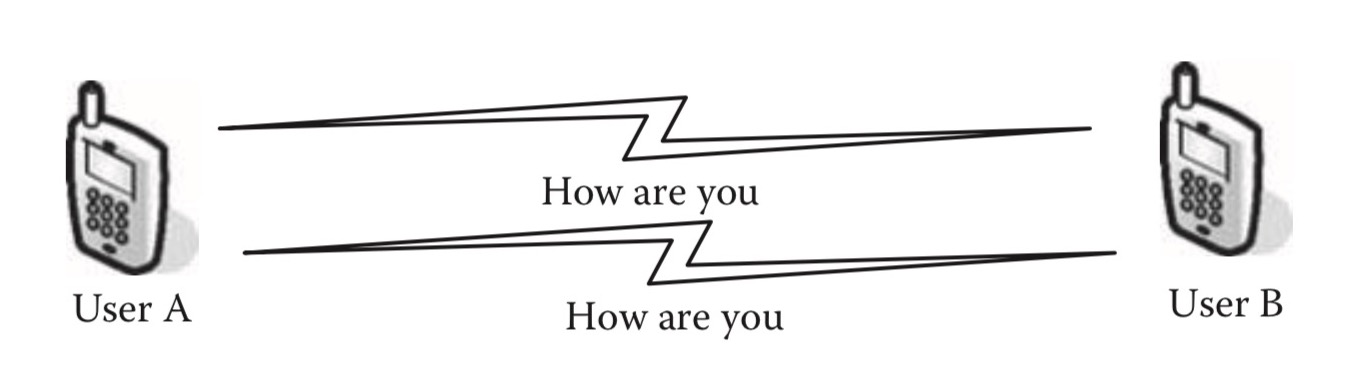
\includegraphics[width=0.7\textwidth]{ptt}
\caption{ارتباط کاملاً دوطرفه\nf ی بی\nf سیم}
\label{ptt}
\end{figure}  

سیستم \lr{IMS}، قابلیت پشتیبانی از \lr{PTT} را دارد. سرویس \lr{PTT} در بستر شبکه\nf ی سلولی، \lr{PoC}\RTLfootnote{\lr{PTT over Cellular}} نام دارد. با استفاده از \lr{PoC}، کاربران تلفن همراه می\nf توانند از سرویس \lr{PTT} بهره\nf مند شوند. همچنین، سیستم \lr{PoC} سرویس\nf های جدیدی نیز ارائه می\nf کند. از قابلیت\nf های اصلی \lr{PoC} می\nf توان به موارد زیر اشاره کرد \cite{weboma}:

\begin{itemize}
\item ارسال محتوای چندرسانه\nf ای(\lr{Push to Video}) علاوه بر ارسال صوت
\item ارتباط با سرویس\nf های کنونی \lr{PTT}
\item ایجاد جلسه\nf ی \lr{PoC} بین ماشین و کاربر
\item \lr{PoC Box}(برای ذخیره کردن مدیای مبادله\nf شده)
\end{itemize}


